\documentclass[Protokollheft.tex]{subfiles}
\begin{document}
\chapter{Grundlagen der Methode der Finiten Integration 1}
%--------------- Start Vorbereitungsaufgaben ---------------
\section{Vorbereitungsaufgaben}
    {\subsection{Überzählige Kanten}}

% --> Aufgabe
        \begin{framed}
	\noindent \textbf{1.} Skizzieren Sie ein zweidimensionales kartesisches Gitter mit
        $3\times 4$ Punkten und tragen Sie alle Kantenindizes für die $x$-
        und $y$-Kanten nach dem kanonischen Indizierungsschema aus Gl.~(2.5) ein. Machen Sie sich klar, welche Indizes zu
        nicht existierenden Kanten gehören und markieren Sie diese.\label{exer:edgeIndices}
\end{framed}

\emph{Fügen Sie hier Ihre Lösung ein}

% --> Aufgabe
        \begin{framed}
	\noindent \textbf{2.} \label{vorb:formel} Überlegen Sie sich für ein $N_x\times N_y$-Gitter eine Formel für die
        Anzahl der Indizes, zu denen keine Kanten gehören. Geben Sie diese Formel auch für den Sonderfall
        $N_{xy}=N_x=N_y$ in Abhängigkeit von $N_{\text{P}}=N_{xy}^2$ an. Geben Sie darüber hinaus auch eine Formel an, um die Indizes aller Geisterkanten nach dem kanonischen Indizierungsschema zu berechnen.\label{exer:nrOfGhostEdges}
\end{framed}

\emph{Fügen Sie hier Ihre Lösung ein}

%
    {\subsection{Dreiecksgitter}}
    Gegeben sind die beiden Dreiecksgitter in Abb.~\ref{fig:tetmesh}, \textbf{wobei
    zunächst nur das linke Gitter betrachtet werden soll.}
  \begin{figure}[htb]
    \centering
    \begin{subfigure}{0.49\textwidth}
        \centering
        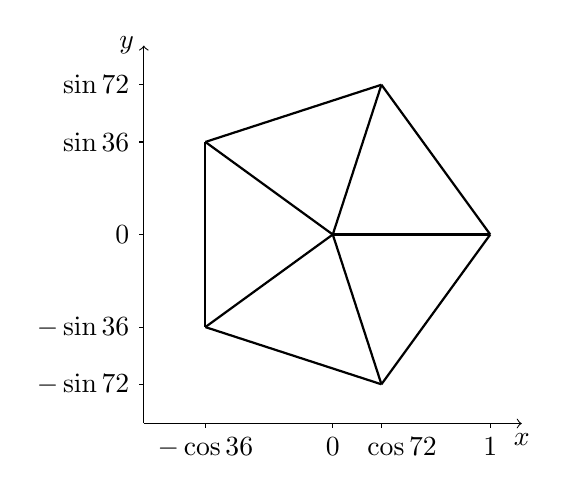
\begin{tikzpicture}[scale=2]
	% Punkte
	\coordinate (axes) at (-1.2,-1.2);
	\coordinate  (c1) at (0,0);
	\coordinate  (c2) at (72:1);
	\coordinate (c3) at (0:1);
	\coordinate (c4) at (-72:1);
	\coordinate (c5) at (-144:1);
	\coordinate (c6) at (144:1);
	\node [left] (n1) at (c1) {};
	\node [above] (n2) at (c2) {};
	\node [right] (n3) at (c3) {};
	\node [below] (n4) at (c4) {};
	\node [left] (n5) at (c5) {};
	\node [left] (n6) at (c6) {};

	% Axen
	\draw [->](axes) -- +(2.4,0) node [below] {$x$};	
	\draw (axes |- c2) -- +(-0.03,0) node [left] {\(\sin 72\degree\)};
	\draw (axes |- c6) -- +(-0.03,0) node [left] {\(\sin 36\degree\)};
	\draw (axes |- c1) -- +(-0.03,0) node [left] {\(0\)};
	\draw (axes |- c5) -- +(-0.03,0) node [left] {\(- \sin 36\degree\)};
	\draw (axes |- c4) -- +(-0.03,0) node [left] {\(-\sin 72\degree\)};
	\draw [->](axes) -- +(0,2.4) node [left] {$y$};
	\draw (axes -| c5) -- +(0,-0.03) node [below] {\(-\cos 36\degree\)};
	\draw (axes -| c1) -- +(0,-0.03) node [below] {\(0\)};
	\draw (axes -| c4) -- +(0,-0.03) node [below right,xshift=-2ex] {\(\cos 72\degree\)};
	\draw (axes -| c3) -- +(0,-0.03) node [below] {\(1\)};

	\begin{scope}[thick]
		% Kanten
		\draw (c1) -- node [auto] {} +(c3);
		\draw (c1) -- node [auto] {} +(c4);
		\draw (c1) -- node [auto] {} +(c5);
		\draw (c1) -- node [auto] {} +(c6);
		\draw (c1) -- node [auto] {} +(c2);
		
		\draw (c2) -- node [auto] {} (c3);
		\draw (c3) -- node [auto] {} (c4);
		\draw (c4) -- node [auto] {} (c5);
		\draw (c5) -- node [auto] {} (c6);
		\draw (c6) -- node [auto] {} (c2);
	\end{scope}
\end{tikzpicture}
            
    \end{subfigure}
    \begin{subfigure}{0.49\textwidth}
        \centering
        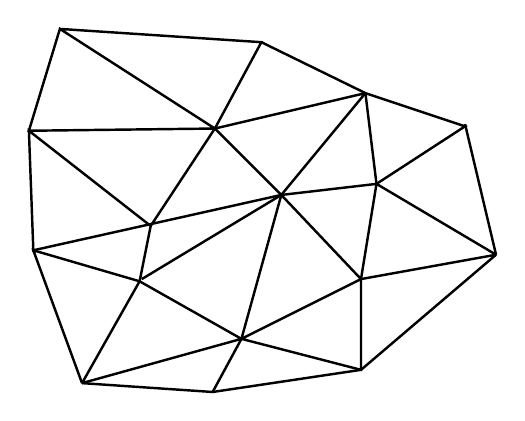
\begin{tikzpicture}[y=0.80pt,x=0.80pt,yscale=-1, inner sep=0pt, outer sep=0pt]
  % path
  \path[draw=black,line join=miter,line cap=butt,miter limit=2.61,line
    width=0.882pt] (293,610) -- (319,564) --
    (365,590) -- (293,610) -- cycle;

  % path
  \path[draw=black,line join=miter,line cap=butt,miter limit=2.61,line
    width=0.882pt] (320,563) -- (383,525);

  % path
  \path[draw=black,line join=miter,line cap=butt,miter limit=2.61,line
    width=0.882pt] (365,590) -- (419,563) --
    (419,604) -- (365,590) -- (383,525) --
    (419,563);

  % path
  \path[draw=black,line join=miter,line cap=butt,miter limit=2.61,line
    width=0.882pt] (293,610) -- (271,550) --
    (319,564);

  % path
  \path[draw=black,line join=miter,line cap=butt,miter limit=2.61,line
    width=0.882pt] (383,525) -- (271,550) --
    (269,496) -- (324,539) -- (353,495) --
    (383,525);

  % path
  \path[draw=black,line join=miter,line cap=butt,miter limit=2.61,line
    width=0.882pt] (319,564) -- (324,539);

  % path
  \path[draw=black,line join=miter,line cap=butt,miter limit=2.61,line
    width=0.882pt] (383,525) -- (421,479) --
    (353,495) -- (269,496) -- (283,450) --
    (353,495) -- (374,456) -- (283,450);

  % path
  \path[draw=black,line join=miter,line cap=butt,miter limit=2.61,line
    width=0.882pt] (374,456) -- (421,479)(426,520)
    -- (419,563);

  % path
  \path[draw=black,line join=miter,line cap=butt,miter limit=2.61,line
    width=0.882pt] (383,525) -- (426,520) --
    (421,479);

  % path
  \path[draw=black,line join=miter,line cap=butt,miter limit=2.61,line
    width=0.882pt] (293,610) -- (352,614) --
    (365,590);

  % path
  \path[draw=black,line join=miter,line cap=butt,miter limit=2.61,line
    width=0.882pt] (419,604) -- (352,614);

  % path
  \path[draw=black,line join=miter,line cap=butt,miter limit=2.61,line
    width=0.882pt] (426,520) -- (480,552) --
    (419,563);

  % path
  \path[draw=black,line join=miter,line cap=butt,miter limit=2.61,line
    width=0.882pt] (419,604) -- (480,552);

  % path
  \path[draw=black,line join=miter,line cap=butt,miter limit=2.61,line
    width=0.882pt] (421,479) -- (466,494) --
    (426,520);

  % path
  \path[draw=black,line join=miter,line cap=butt,miter limit=2.61,line
    width=0.882pt] (480,552) -- (466,493);

\end{tikzpicture}

    \end{subfigure}
    \caption{Dreiecksgitter von zwei verschiedenen Rechengebieten.}
    \label{fig:tetmesh}
  \end{figure}
    %

% --> Aufgabe
        \begin{framed}
	\noindent \textbf{3.} Nummerieren Sie die Flächen und Kanten des Gitters beliebig und ordnen
                    Sie den Kanten eine Orientierung zu.\label{exer:triangleOrderedNumbering}
\end{framed}

\emph{Fügen Sie hier Ihre Lösung ein}

% --> Aufgabe
        \begin{framed}
	\noindent \textbf{4.} Erstellen Sie die Punkteliste (3-spaltige Tabelle mit Index, $x$-Koordinaten und $y$-Koordinaten). Stellen Sie auch die Indexlisten Kanten-zu-Knoten und Flächen-zu-Kanten auf (auch Inzidenzen genannt).
                    Beachten Sie dabei die Orientierung der Kanten und Flächen. Die Kanten sind von Punkt 1
                    zu Punkt 2 gerichtet. Bei der Flächen-zu-Kanten-Inzidenz werden Kanten, die gegen die
                    Umlaufrichtung der Fläche zeigen, mit einem negativen Vorzeichen vor dem Index gekennzeichnet.\label{exer:incidences}
\end{framed}

\emph{Fügen Sie hier Ihre Lösung ein}

% --> Aufgabe
        \begin{framed}
	\noindent \textbf{5.} Erstellen Sie aus der Kanten-zu-Knoten-Inzidenz die Gradientenmatrix $\gradfit$.
                    Gehen Sie von einem Potentialvektor {\boldmath $\varphi$}
                    der Dimension $N_\text{P}$ aus, der die Werte einer
                    Potentialfunktion in allen Gitterpunkten enthält. Legen Sie
                    die Matrix $\gradfit$ so fest, dass die Multiplikation $-\mbox{\boldmath
                    $\gradfit \varphi$}$ gerade den Vektor $\efit$ ergibt, was der
                    kontinuierlichen Formel $\vec{E}=-\grad\varphi$ entspricht.\label{exer:gradfit}
\end{framed}

\emph{Fügen Sie hier Ihre Lösung ein}

% --> Aufgabe
        \begin{framed}
	\noindent \textbf{6.} Konstruieren Sie mithilfe der Flächen-zu-Kanten-Inzidenz die Curlmatrix $\curlfit$.\\
              Zur Erinnerung: $\curlfit \efit = - \frac{\text{d}}{\text{d}t} \bfit$.\label{exer:curlfit}
\end{framed}

\emph{Fügen Sie hier Ihre Lösung ein}

% --> Aufgabe
        \begin{framed}
	\noindent \textbf{7.} Überprüfen Sie, ob genau wie im kontinuierlichen Fall die Beziehung $\rot\grad=0$ auch für die aufgestellten diskreten Matrizen $\curlfit\gradfit={\textbf{0}}$ gilt.\label{exer:rotgradZero}
\end{framed}

\emph{Fügen Sie hier Ihre Lösung ein}

%
    {\subsection{Duale Gitter}}
    Ein mögliches Gestaltungsprinzip für das duale Gitter eines
    Dreiecksgitters resultiert aus der Forderung, dass die dualen
    Kanten die normalen Flächen (2D = normale Kanten) orthogonal
    durchstoßen. Es wird daher versucht, die dualen Kanten aus den
    \emph{Mittelsenkrechten} der Dreiecke zu konstruieren, die sich
    bekanntermaßen in einem Punkt -- dem neuen dualen Gitterpunkt --
    schneiden. Voraussetzung für dieses Vorgehen ist jedoch, dass
    der Schnittpunkt der Mittelsenkrechten auch innerhalb des Dreiecks
    liegt, was nicht immer erfüllt ist.\\
    \subsection{Ab hier sollen beide Gitter aus Abb.~\ref{fig:tetmesh} betrachtet werden.}

% --> Aufgabe
        \begin{framed}
	\noindent \textbf{8.} Zeichnen Sie das orthogonale duale
        Gitter ein, wenn möglich nach der oben beschriebenen
        Konstruktionsvorschrift. Markieren Sie die dualen
        Gitterkanten, die die Eigenschaft der Orthogonalität nicht mehr
        erfüllen.\label{exer:drawDualGrid}
\end{framed}

\emph{Fügen Sie hier Ihre Lösung ein}

% --> Aufgabe
        \begin{framed}
	\noindent \textbf{9.}
        Überlegen Sie sich, wie $N_\text{V}$, $N_\text{A}$, $N_\text{L}$ und $N_\text{P}$
        mit den entsprechenden Größen des dualen Gitters $\widetilde N_\text{V}$,
        $\widetilde N_\text{A}$, $\widetilde N_\text{L}$ und $\widetilde N_\text{P}$ im Fall
        von 3D-Gittern zusammenhängen. Besonderheiten am Rand sind hierzu zu vernachlässigen.
        Wie verhalten sich die Größen im Fall von 2D-Gittern?\label{exer:primaryDualCorrespondence}
\end{framed}

\emph{Fügen Sie hier Ihre Lösung ein}

\section{Aufgaben während der Praktikumssitzung}

    {\subsection{Datenstruktur, Visualisierung des Gitters}}

% --> Aufgabe
        \begin{framed}
	\noindent \textbf{1.} Schreiben Sie eine Methode zur Abspeicherung dreidimensionaler,
                    kartesischer Gitter in einem \lstinline{struct}
                    \begin{align}
                        \lstinline{[msh] = cartMesh(xmesh, ymesh, zmesh)}
                    \end{align}
                    und verwenden Sie die Definitionen der Eingangsparameter
                    aus Abschnitt 2.2.3. Die Struktur \lstinline{msh} hält nach Aufruf dieser Funktion das durch \lstinline{xmesh}, \lstinline{ymesh} und \lstinline{zmesh} definierte Gitter.
                    Für spätere Routinen muss in \lstinline{msh} auch die Gitterpunkteanzahl in
                    jede Raumrichtung, d.\,h. \lstinline{nx}, \lstinline{ny} und \lstinline{nz}, abgespeichert werden.\label{exer:cartMesh}
\end{framed}

\emph{Fügen Sie hier Ihre Lösung ein}

% --> Aufgabe
        \begin{framed}
	\noindent \textbf{2.} Implementieren Sie die Methode
                    \begin{align}
                        \lstinline{plotMesh(msh)} \; ,
                    \end{align}
                    welche ein übergebenes kartesisches Gitter \lstinline{msh} visualisiert. Verwenden
                    Sie hierzu den \lstinline{line}-Befehl und eine 3-fach Schleife über die Indizes $i,j,k$.\label{exer:plotMesh}
\end{framed}

\emph{Fügen Sie hier Ihre Lösung ein}

% --> Aufgabe
        \begin{framed}
	\noindent \textbf{3.} Nutzen Sie \lstinline{cartMesh} zur Erzeugung eines nicht äquidistanten Gitters mit \{3,4,5\} Punkten in \{$x$,$y$,$z$\}-Richtung und visualisieren Sie es mit \lstinline{plotMesh}. Nutzen Sie hierfür die bereits gegebene Datei \lstinline{exampleMesh.m}.\label{exer:createVisualizeMesh}
\end{framed}

\emph{Fügen Sie hier Ihre Lösung ein}

%
    {\subsection{Die topologischen Matrizen $\curlfit$, $\curldfit$, $\divfit$ und $\divdfit$}}

% --> Aufgabe
        \begin{framed}
	\noindent \textbf{4.} Schreiben Sie eine Methode
                    \begin{align}
                        \lstinline{[c, s, st] = geoMats(msh)} \; ,
                    \end{align}
                    die die Operatormatrizen für ein kanonisches, kartesisches
                    Gitter \lstinline{msh} erzeugt. Die Rückgabewerte
                    \lstinline{c}, \lstinline{s} und \lstinline{st}
                    sind die Matrizen $\curlfit$, $\divfit$ und $\divdfit$
                    und entsprechend Abschnitt 2.2.7 definiert. Diese werden mithilfe der
${\mathbf{P_\xi}}$-Matrizen erzeugt.
                    Wieso ist es nicht sinnvoll, $\curldfit$ und $\gradfit$ zurückzugeben?\\
                    \ \\
                    {\textbf{Hinweis:}} Schon bei mittleren Problemgrößen muss hier
                    unbedingt mit \matlab{s} speziellem Speicherformat für
                    \emph{dünnbesetzte} Matrizen gearbeitet werden (Befehle wie
                    \lstinline{sparse}, \lstinline{speye}, usw.) Im Allgemeinen geben
                    \matlab-Befehle immer dann Matrizen im \lstinline{sparse}-Format
                    zurück, wenn \emph{alle} ihre Argumente ebenfalls \lstinline{sparse}
                    sind. Mehr zu diesem Thema ist in der \matlab-Dokumentation zu finden.\label{exer:geoMats}
\end{framed}

\emph{Fügen Sie hier Ihre Lösung ein}

% --> Aufgabe
        \begin{framed}
	\noindent \textbf{5.} Lassen Sie sich die Matrizen für eine kleine Problemgröße ($N_{\text{P}}<50$) direkt
                    ausgeben und visualisieren Sie die Matrizen für eine mittlere
                    Problemgröße ($N_{\text{P}}<5000$) mit dem Befehl \lstinline{spy}. Welche speichertechnisch günstige
                    Eigenschaft würde ohne das kanonische Indizierungsschema verloren gehen?
                    Ermitteln Sie wie viel Speicherplatz jeweils von \matlab benötigt wird
                    (\lstinline{sparse} und \lstinline{full}-Format). Legen Sie für die Ausarbeitung eine Tabelle mit dem jeweils benötigten Speicherplatz an. Nutzen Sie für diese Tests die bereits gegebene Datei \lstinline{exampleSparse.m}.\label{exer:spyStorage}
\end{framed}

\emph{Fügen Sie hier Ihre Lösung ein}

% --> Aufgabe
        \begin{framed}
	\noindent \textbf{6.} Berechnen Sie
                    \begin{enumerate}
                        \item $\curlfit\, (-\divdfit^{\text{T}})$ und
                        \item $\divfit\, \curlfit$ bzw. $\divdfit\, \curldfit$ \; .
                    \end{enumerate}
                    Was bedeutet das für die topologischen Matrizen in Hinblick
                    auf die jeweiligen analytischen Operatoren? Erinnern Sie sich, welche analytischen Operatoren den jeweiligen Matrizen entsprechen.\label{exer:CG_SC}
\end{framed}

\emph{Fügen Sie hier Ihre Lösung ein}

{\subsection{Unbelegte Kantenelemente}}

% --> Aufgabe
        \begin{framed}
	\noindent \textbf{7.} Als Fortführung von Aufgabe 2 aus der Vorbereitung
                    konstruieren Sie eine Routine, die die überzähligen Kanten erfasst.
                    \begin{align}
                        \lstinline{edg = boundEdg(msh)}
                    \end{align}
                    gibt demnach für ein gegebenes Gitter \lstinline{msh} einen Vektor \lstinline{edg} zurück, der
                    entsprechend der kanonischen Indizierung \lstinline{true} für normale und \lstinline{false}
                    für die überzähligen Kanten enthält.\\
                    \ \\
                    {\textbf{Hinweis:}} Benötigt wird in diesem Versuch nur der zweidimensionale Fall \lstinline{nz=1}, jedoch ist es für spätere Versuche hilfreich auch den dreidimensionalen Fall zu implementieren. Zusätzlich ist es sinnvoll, Erfahrungen mit Vektoroperationen zu sammeln, da diese in \matlab in der Regel schneller sind als Schleifen. Das \lstinline{logical}-Format (in anderen Programmiersprachen auch als \lstinline{boolean} bekannt) hat den Vorteil, dass nur $1$ Byte (im Vergleich zu $8$ Bytes für \lstinline{double}) pro Eintrag benötigt wird.\label{exer:boundEdg}
\end{framed}

\emph{Fügen Sie hier Ihre Lösung ein}

% --> Aufgabe
        \begin{framed}
	\noindent \textbf{8.} Zählen Sie mit \lstinline{boundEdg} die unbelegten Kanten und vergleichen Sie Ihr Ergebnis mit
                    der Formel aus der 2. Vorbereitungsaufgabe, indem Sie die relative Anzahl der
                    unbelegten Kanten (inkl. Geisterkanten in $z$-Richtung) über die Anzahl aller Kanten für ein zweidimensionales Gitter \lstinline{msh} mit $N_{xy}=N_x=N_y$ darstellen. \lstinline{plotBoundEdg} soll diese Aufgaben dann in einem Skript zusammenfassen.\label{exer:plotBoundEdg}
\end{framed}

\emph{Fügen Sie hier Ihre Lösung ein}

{\subsection{Einprägen gegebener Feldverteilungen}}

% --> Aufgabe
        \begin{framed}
	\noindent \textbf{9.} Schreiben Sie eine Methode, die für ein
        vorgegebenes kontinuierliches $\vec{E}$-Feld \lstinline{field}
        die entsprechenden integralen Zustandsgrößen \lstinline{fieldBow}
        in einem 3D-Gitter \lstinline{msh} berechnet und in einem Vektor gemäß
        Gl.~(2.8) abspeichert. Implementieren Sie:
        \begin{align}
            \lstinline{[fieldBow] = impField(msh, field)}
        \end{align}
        {\textbf{Hinweis:}} \lstinline{field} soll hierbei eine \emph{anonymous function} sein, welche den Punkt mit $x$-,$y$- und $z$-Koordinate übergeben bekommt und einen Vektor mit $x$-,$y$- und $z$-Komponente zurückgibt. Zum Beispiel:
        \begin{center}
            \lstinline{field = @(x,y,z)([1./x.^2, 0.01*x, y+z])}\\
            Aufruf mit \lstinline{field(1, 3, 4.5)} oder \lstinline{field([3,6]', [1,3]', [2,4]')} \; .
        \end{center}
        Werten Sie für die notwendige Integration über eine Kante das gegebene Feld an den Kantenmittelpunkten aus und multiplizieren Sie den Wert mit
        der Kantenlänge anstatt das Feld tatsächlich zu integrieren.\label{exer:impField}
\end{framed}

\emph{Fügen Sie hier Ihre Lösung ein}

% --> Aufgabe
\newpage
        \begin{framed}
	\noindent \textbf{10.} Verwenden Sie Ihre Methode \lstinline{impField} um folgende Felder zu diskretisieren:
        \begin{enumerate}
            \item $\Ev(\vec r) = \frac{5}{2}\, \ex - 1,\!3\, \ey + 2\, \ez,$
            \item $\Ev(\vec r) = 3\, \sin\! \left(\frac{\pi}{x_\text{max}-x_\text{min}}\, (x-x_\text{min}) \right)\, \ey$ ,
        \end{enumerate}
        wobei die Einheiten hier vernachlässigt werden. Mit Hilfe der vorgegebenen Routine \lstinline{plotEdgeVoltage} sollen Sie Ihre Implementation optisch verifizieren. Fassen Sie diese Aufgabe in einem Skript \lstinline{plotImpField} zusammen.\label{exer:plotImpField}
\end{framed}

\emph{Fügen Sie hier Ihre Lösung ein}

\section{Fragen zur Ausarbeitung}

% --> Aufgabe
\begin{framed}
	\noindent \textbf{1.} In den Vorbereitungsaufgabe zum dualen Gitter wurden
Besonderheiten am Rand des Rechengebietes vernachlässigt.

Wie sollte das duale Gitter am Rand gewählt werden, damit die magnetische
Randbedingung automatisch erfüllt ist. Machen Sie eine kleine Skizze
für ein einfaches zweidimensionalen kartesisches Gitter sowie für
das Dreiecksgitter aus Bild \ref{fig:tetmesh} a). Ist diese Wahl
des dualen Gitters am Rand immer notwendig?\label{exer:autoHomNeumann}
\end{framed}

\emph{Fügen Sie hier Ihre Lösung ein}



\section{Fazit}
\emph{Fügen Sie hier Ihre Lösung ein}

\end{document}
